%&pdflatex
\documentclass[11pt, twocolumn]{article}
\usepackage{caption}
\usepackage{chemformula}
\usepackage{float}
\usepackage{fullpage}
\usepackage{graphicx}
\usepackage{hyperref}
\usepackage{microtype}
\usepackage{minted}
\usepackage{setspace}
\usepackage[caption=false]{subfig}
\usepackage{titlesec}


\captionsetup{justification=centering, font=footnotesize}
\hbadness=99999  % or any number >=10000
\graphicspath{{../figures/}}
\titleformat{\section}{\normalfont\scshape}{\thesection}{1em}{}
\titleformat{\subsubsection}{\normalfont\scshape}{\thesection}{1em}{}

\newcommand*{\nolink}[1]{%
\begin{NoHyper}#1\end{NoHyper}%
}

\newenvironment{absolutelynopagebreak}
{\par\nobreak\vfil\penalty0\vfilneg
 \vtop\bgroup}
{\par\xdef\tpd{\the\prevdepth}\egroup
 \prevdepth=\tpd}


\begin{document}

\title{Molecular Dynamics Simulation of the D102A Variant of Chymotrypsin
Supports Asp-His Hydrogen Bonding Conformational Restraint}
\author{David Li\\\href{mailto:dzli@jhu.edu}{\nolinkurl{dzli@jhu.edu}}
\and Patrick Fleming\\\href{mailto:Pat.Fleming@jhu.edu}{\nolinkurl{Pat.Fleming@jhu.edu}}}
\date{\today}
\maketitle

\section{Introduction}
Almost one third of all proteases can be classified as serine proteases
~\cite{hedstrom02}. These proteins are named for the nucleophilic Ser
residue at the active site. Serine proteases fall into two broad categories
based on their structure: chymotrypsin-like (trypsin-like) or subtilisin-like
~\cite{madala10}. Chymotrypsin-like proteases are the most abundant in
nature and can be found in eukaryotes, prokaryotes, archae, and viruses. They
are involved in many critical physiological processes, such as hemostasis,
apoptosis, digestion, and reproduction~\cite{hedstrom02}.

In order to hydrolyze a peptide bond, these well-studied enzymes must overcome
three major mechanistic barriers: (i) amide bonds are extremely stable due to
electron donation from the amide nitrogen to the carbonyl; (ii) water is a poor
nucleophile and proteases always activate water via a general base; (iii) and
amines are poor leaving groups because proteases protonate the amine prior to
expulsion~\cite{hedstrom02}.

To overcome these three reaction barriers, serine proteases contain a group
of three residues called the catalytic triad that use hydrogen bonding to
increase reaction favorability. In chymotrypsin, the triad is composed of
serine, histidine, and aspartate, and is part of a larger hydrogen bonding
network~\cite{hedstrom02}.

\begin{figure}[H]
    \subfloat[Wild-Type\label{fig:triad_wt}]{
        \frame{
            \includegraphics[trim={0 0 0 1}, clip, width=0.45\textwidth]
                {wt_conformation1.png}
        }
    }

    \subfloat[D102A variant\label{fig:triad_d102a}]{
        \frame{
            \includegraphics[trim={0 0 0 1}, clip, width=0.45\textwidth]
                {d102a_conformation1.png}
        }
    }
    \caption{Conformation of catalytic triad structure in wild-type and D102A
    variant of chymotrypsin.}\label{fig:triad}
\end{figure}

Mutagenesis experiments of catalytic
triad residues show decreased catalytic activity; substitution of Ser-195 or
His-57 with alanine effectively disables the triad~\cite{hedstrom02}. For
this project, we test the hypothesis that the Asp-His hydrogen bond restrains
the conformational flexibility of the His ring so that it can more strongly
hydrogen bond to serine, thus activating serine for a nucleophilic attack.

To test this, two all-atom molecular dynamics simulations of two chymotrypsin
series variants were carried out: the wild-type sequence, and with Asp-102
substituted for alanine (mutation D102A). This enabled us to determine rotamer
distributions of the His side chain and the time-dependent frequencies of
His-Ser bond formations.

\section{Methods}

A chymotrypsin from \textit{Bos taurus}
(RCSB PDB ID:\@ \href{http://www.rcsb.org/pdb/explore.do?structureId=1ggd}{1GGD})
was used as the starting structure, with an additional calcium atom added to
stabilize the enzyme. The charged form of aspartate (ASP) and the neutral form
of histidine (HSD) were used when building the system with VMD 1.9.3. After
stabilizing, VMD was used to neutralize the system with water and 0.2M \ch{KCl}.
The D102A system was created using the same parameters, solvation, and
neutralization as the wild-type system but the catalytic triad aspartate was
mutated to an alanine residue.

After these steps, the wild-type system contained 16142 atoms and the D102A
system contained 16138 atoms. Both systems were centered about the origin and
the B-factor of the protein atoms was set to 1.00. The minimum and maximum
coordinates of the system were then calculated in order to set the bounding
box for periodic boundary conditions with side length of 60\AA{} in all 3
coordinate directions.

The systems were simulated in an isobaric ensemble (NPT conditions), with a
temperature of 298.15 K and pressure of 1 atmosphere. To control temperature,
Langevin dynamics were used with a coupling coefficient
\(\gamma = 1 \mathrm{ps}^{-1}\). To maintain constant pressure, a Langevin
piston Nos\'e-Hoover method was used in NAMD with a piston period of
100 fs and a piston decay of 50 fs~\cite{namd05}. Finally, the CHARMM
force field was used to calculate interatomic forces with a cutoff distance
of 12\AA{}.

Both simulations were run through three equilibration runs and one production
run. The first equilibration run had a 1 fs time-step and was run for 10000
steps (10 ps simulation), and water molecules were free to move around the
fixed protein.
The second equilibration run had a 1 fs time-step and was run for 10000 steps
(10 ps simulation), but in this case both water and protein were free to move.
The third and final equilibration run had a 2 fs time-step and was run for
2500000 steps (5 ns simulation), and again, both water and protein were free
to move.
The production run used a 2 fs time-step and was run for 5000000 steps (10 ns
simulation) with a frame capture every 2 ps for a total of 5000 frames in the
resulting dcd trajectory file.

Simulations were conducted on the JHU Biophysics kirin cluster running Ubuntu
12.04 with 12 computation nodes. Analysis of results was done using VMD 1.9.3
and Python 2.7.13 (NumPy, SciPy, and matplotlib packages).

\section{Results}

Figure~\ref{fig:triad} shows the catalytic triads of the wild-type and mutated
chymotrypsin. Comparing figure~\ref{fig:triad_wt} and
figure~\ref{fig:triad_d102a} shows the loss of three Asp-His hydrogen bonds
in the mutant. These hydrogen bonds are the ones that were hypothesized to
conformationally restrain the histidine.

The root-mean-square deviation (RMSD) of atomic positions of the D102A variant
was determined to be slightly higher than
that of the wild-type variant, with an average of 2.09\AA{} compared to
2.00\AA{}. As seen in Figure~\ref{fig:rmsd}, after about 8 ns of simulation,
the D102A RMSD sharply increases to around 2.5\AA{}, indicative of a loop
flexing out, which can be confirmed from visual inspection of the trajectory.
\begin{figure}[H]
    \centering
        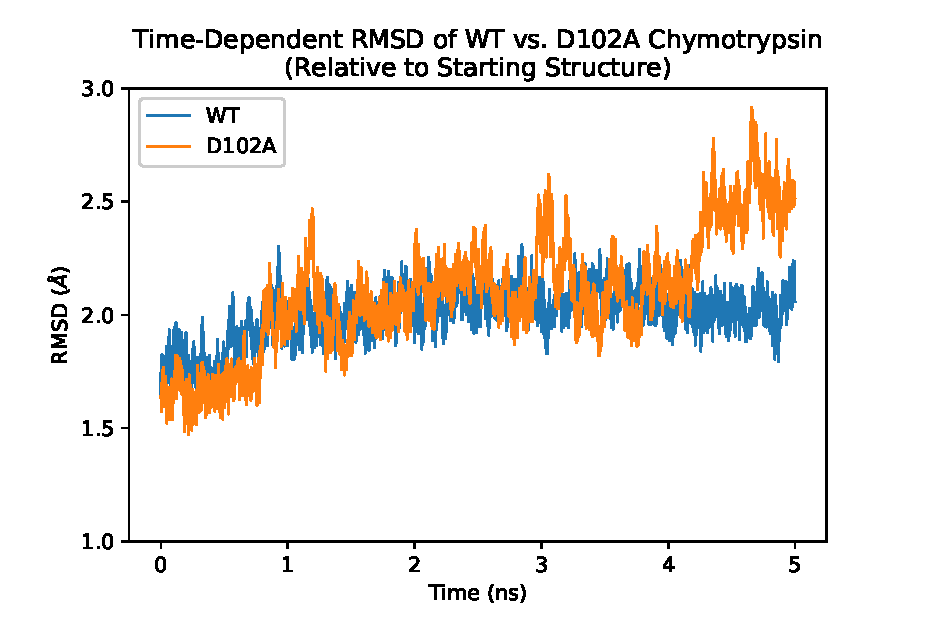
\includegraphics[width=0.49\textwidth]{rmsds.eps}
    \caption{RMSD of wild-type (WT) and D102A simulations.}\label{fig:rmsd}
\end{figure}

\vspace{-20pt}

\begin{figure}[H]
    \centering
        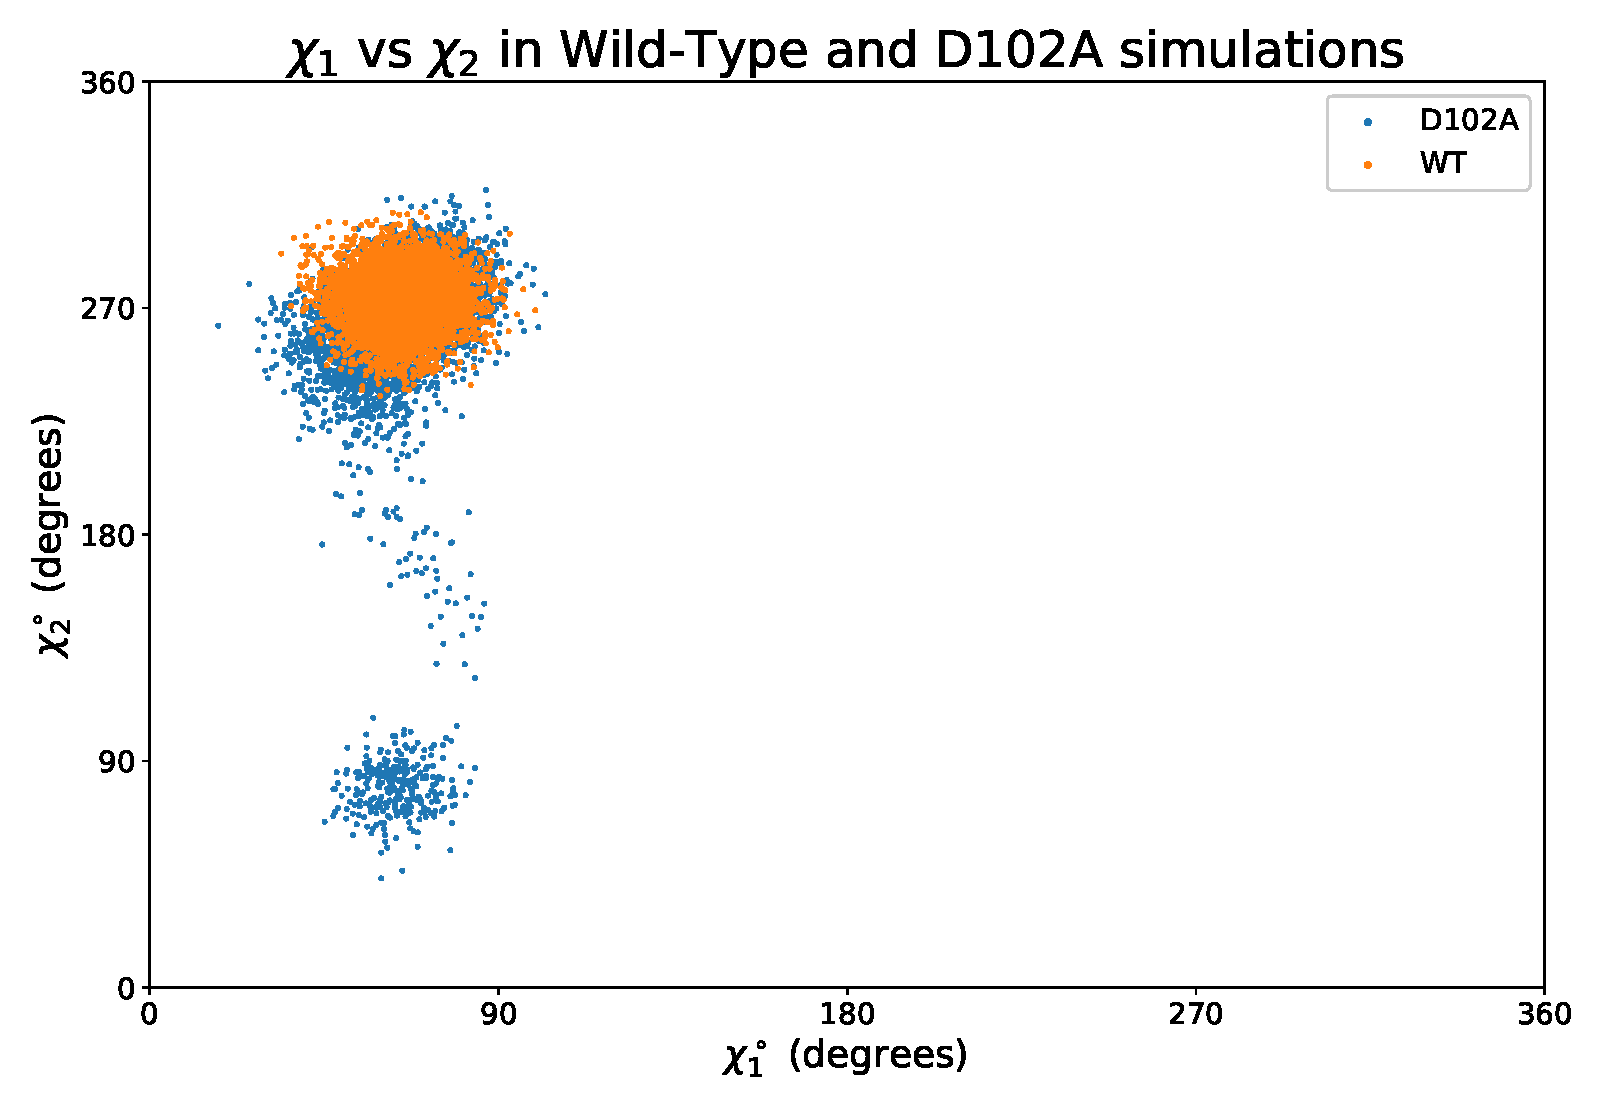
\includegraphics[width=0.49\textwidth]{chi_plot_wt_d102a.eps}
    \caption{Dihedral bond angle distribution for Histidine Side Chains
        in WT and D102A simulations reveals bimodal distribution
        in D102A mutant.}\label{fig:chiplot}
\end{figure}


The dihedral angle between H59 \(\alpha\)-carbon and \(\beta\)-carbon
(\(\chi_1\)) and the dihedral angle between H59 \(\beta\)-carbon and
\(\gamma\)-carbon (\(\chi_2\)) were measured for each frame in the WT and
D102A simulations. As seen in Figure~\ref{fig:chiplot}, the wild-type
chymotrypsin stayed in one region centered around
\((\chi_1, \chi_2) \approx (70^\circ, 270^\circ)\).
In contrast, the D102A variant showed significantly higher variability
in dihedral angles, where the distribution appeared to be bimodal with
two peaks centered around \((\chi_1, \chi_2) \approx (70^\circ, 90^\circ)\)
and \((\chi_1, \chi_2) \approx (70^\circ, 270^\circ)\). Even in the region
centered around \((\chi_1, \chi_2) \approx (70^\circ, 270^\circ)\), the
mutant samples a wider range of bond angles.


\begin{figure}[H]
    \centering
        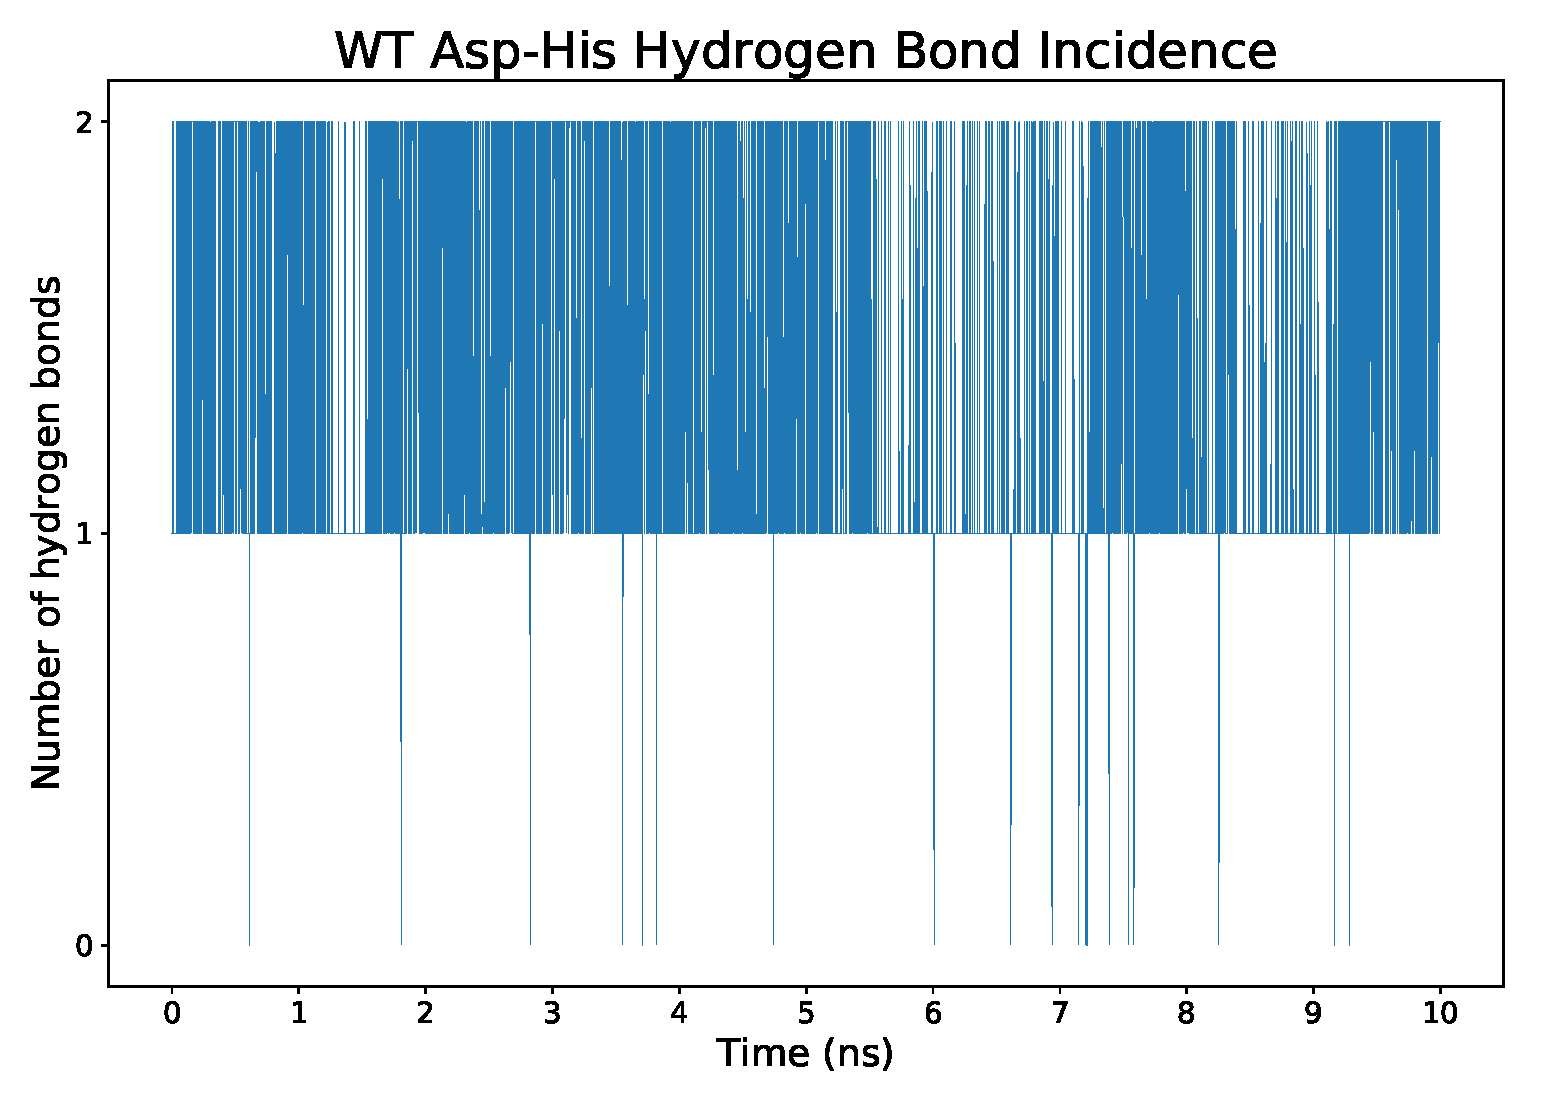
\includegraphics[width=0.49\textwidth]{wt_hbonds_asp_his.eps}
    \caption{Rapid Conversion between 1 and 2 Asp-His hydrogen bonds
        of wild-type chymotrypsin indicates persistent
        bond.}\label{fig:hbond_asp_his}
\end{figure}

For the analysis, hydrogen bonds were defined as a maximum distance of 3.5\AA{}
between donors and accepters with a maximum angle of 45\(^\circ\). Hydrogen
bond incidence can then be plotted versus simulation time -- see
Figures~\ref{fig:hbond_asp_his},~\ref{fig:hbond_his_ser_wt},~\ref{fig:hbond_his_ser_d102a}.
Figure~\ref{fig:hbond_asp_his} demonstrates wild-type Asp-His hydrogen bonds
are relatively stable, terminating infrequently over the entire simulation.
The fluctuations are mostly between 1 and 2 hydrogen bonds (an Asp-His hydrogen
bond exists in 99.6\% of the sampled frames), indicating that the hydrogen
in the histidine was forming and breaking bonds with the oxygen in the
aspartate rapidly.


\begin{figure}[H]
    \centering
        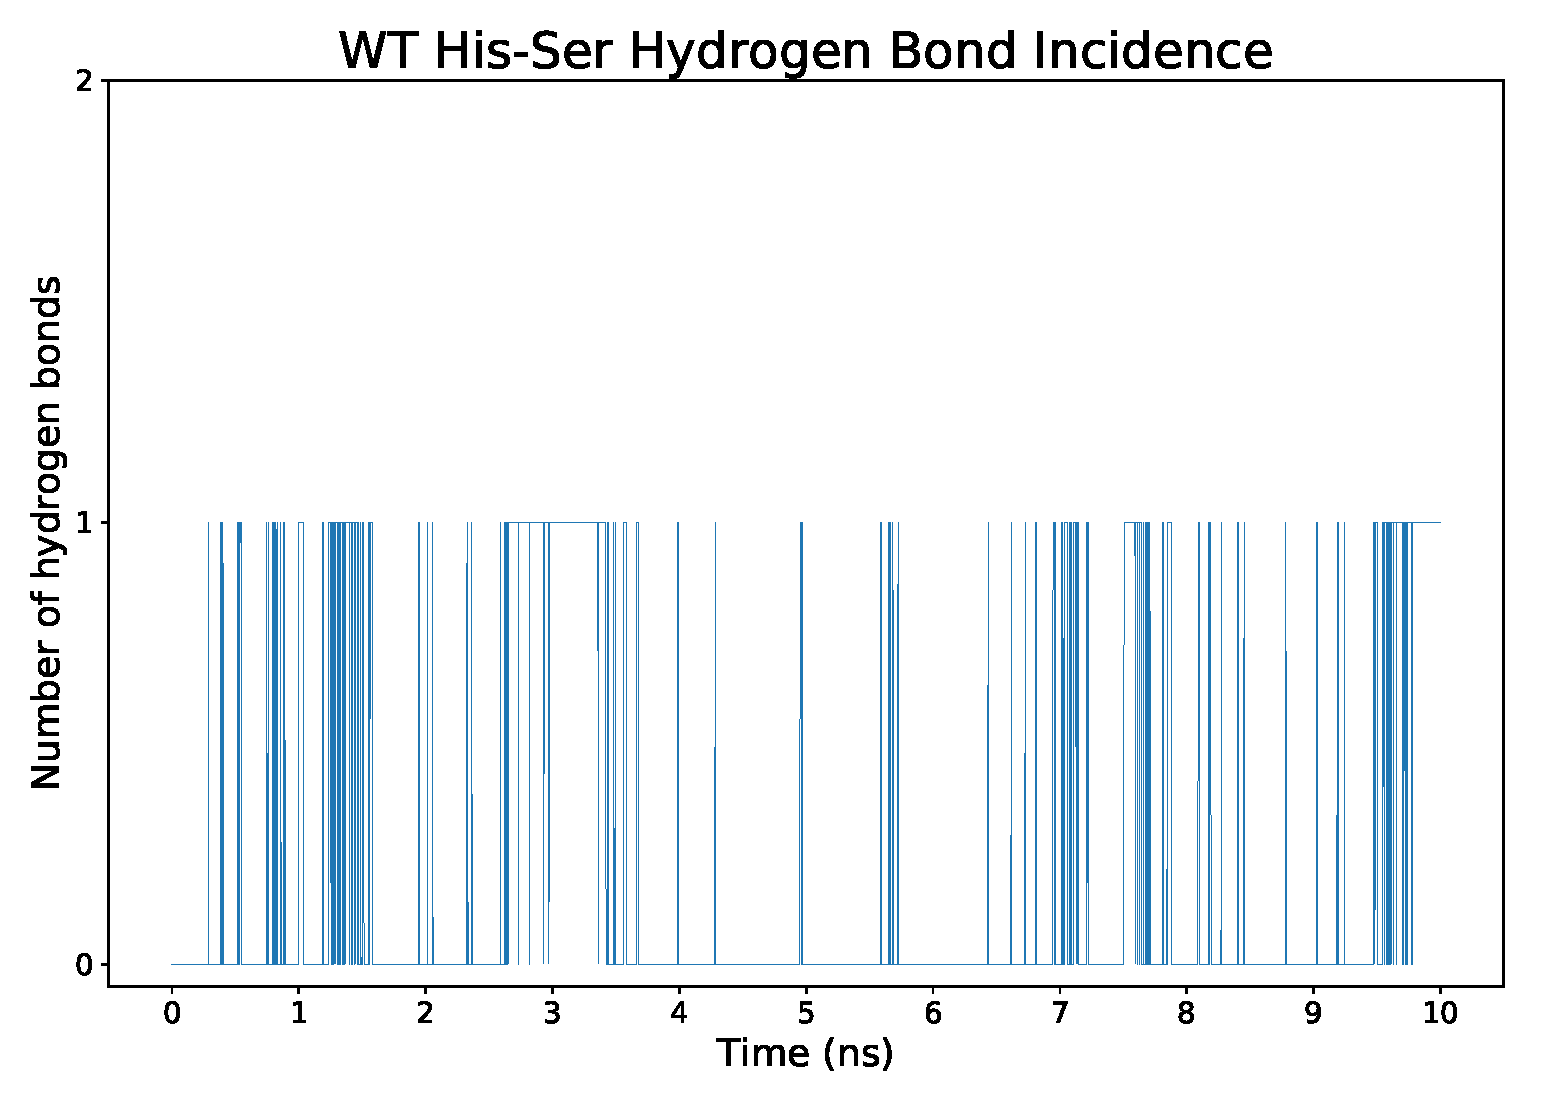
\includegraphics[width=0.49\textwidth]{wt_hbonds_his_ser.eps}
    \caption{Conformations containing a His-Ser hydrogen bond are
        more infrequently sampled than those with a Asp-His
        hydrogen bond. 304 bonds shown.
        }\label{fig:hbond_his_ser_wt}
\end{figure}

Figure~\ref{fig:hbond_his_ser_wt} shows that conformations with the His-Ser
hydrogen bond are more infrequently sampled over the simulation compared to
conformations with a Asp-His hydrogen bond. Quantitatively, 20.3\% of frames
contained a His-Ser hydrogen bond.

% \vspace{70pt}
\begin{figure}[H]
    \centering
        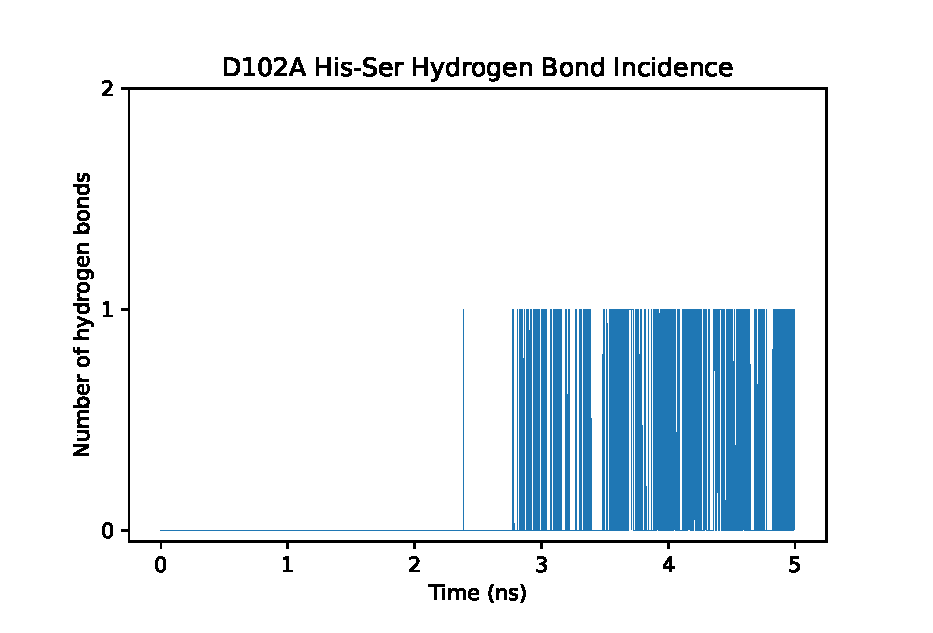
\includegraphics[width=0.49\textwidth]{d102a_hbonds_his_ser.eps}
    \caption{D102A simulation initially samples conformations without hydrogen
        bonding, but suddenly samples such conformations. 139 bonds shown.
        }\label{fig:hbond_his_ser_d102a}
\end{figure}


Interestingly, in
Figure~\ref{fig:hbond_his_ser_d102a} the mutated variant, the histidine
residue initially does not sample conformations with any hydrogen bonds, but
ends up sampling such conformations somewhat frequently. In the first half
of the D102A simulation, only one frame has a His-Ser hydrogen bond. However,
in the second half of the simulation, 27.7\% of the frames contain a His-Ser
hydrogen bond. It seems that the histidine rotated into position and stayed
in position even without aspartate to stabilize it with hydrogen bonds.


His-Ser hydrogen bond lifetimes were also calculated with VMD, and analysis
of the results was done in Python. The wild-type chymotrypsin had an average
bond lifetime of 65.04 ps, while the mutated variant had an average lifetime
of 22.80 ps. The wild-type also had higher maximum bond lifetimes (6 instances
of bond lifetimes over 200 ps, with a maximum of 1930 ps) than the D102A
variant (maximum bond lifetime of 210 ps). Furthermore, an exponential
best-fit line can be fit to the histogram.
Analysis code can be found in Appendix~\ref{code}.

\begin{figure}[H]
    \centering
    \subfloat[Wild-type, 304 bonds measured\label{fig:lifetime_wt}]{
        % \frame{
            \centering
            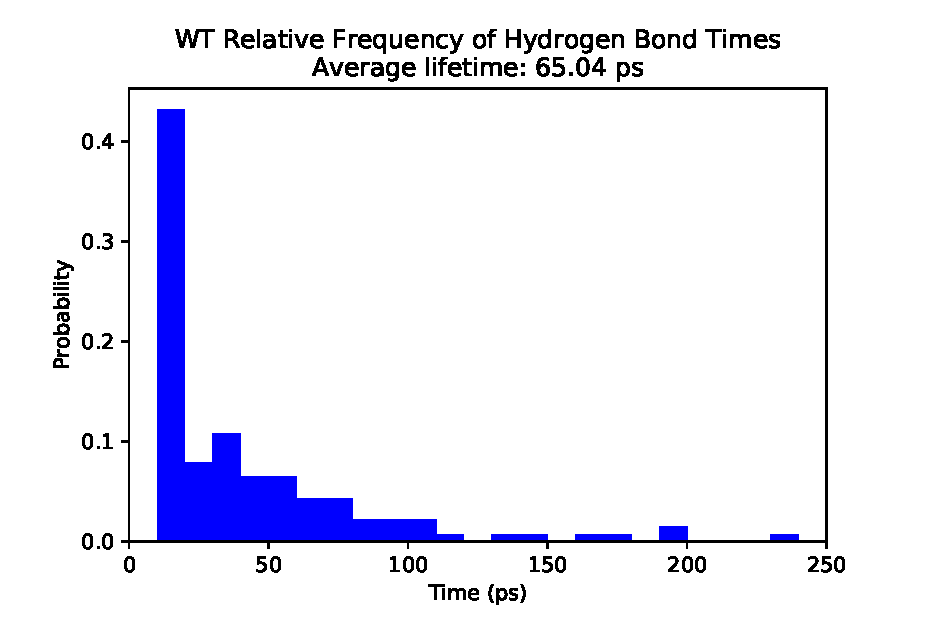
\includegraphics[width=0.49\textwidth]{wt_hbond_times.eps}
        % }
   }

    \subfloat[D102A, 139 bonds measured\label{fig:lifetime_d102a}]{
        % \frame{
            \centering
            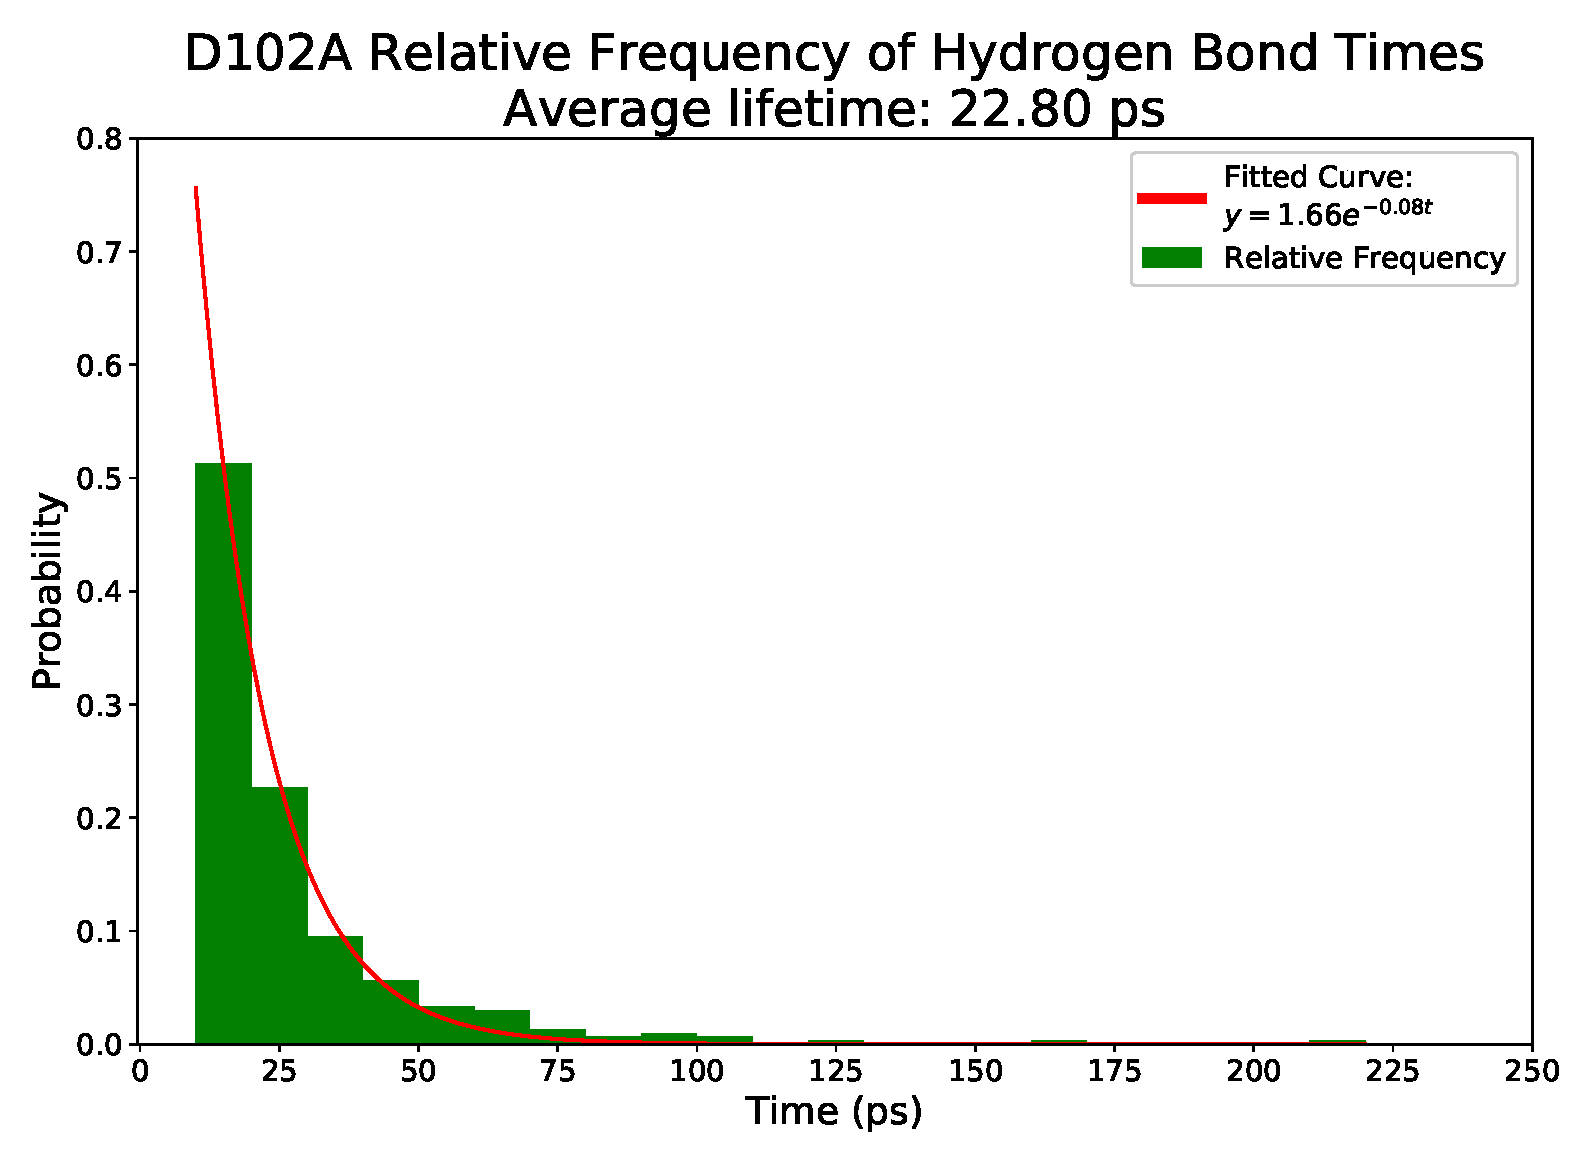
\includegraphics[width=0.49\textwidth]{d102a_hbond_times.eps}
        % }
    }

    \caption{Hydrogen bond lifetimes in simulations of
        (a) Wild-type chymotrypsin and (b) D102A variant
        }\label{fig:hbond_times}
\end{figure}


\newpage
\section{Conclusion}

The data supports the hypothesis that Asp-102 conformationally restrains His-57
to better enable hydrogen bonding between His-57 and Ser-195.
First, the higher RMSD for the D102A from the simulation is evidence of a
greater range of motion and increased flexibility within the D102A variant.
One explanation for this is the lack of two hydrogen bonds at the active site
between residues 57 and 102. However, this isn't strong direct evidence for
the hypothesis because the RMSD is a measure of \textit{all} deviations of
the displacement between the mutant and the starting structure over the course
of the simulation, and is not specific to the active site. Furthermore, the
difference between RMSD is rather small (only 0.09\AA{}), and up until the
sudden jump at 8 ns, the RMSD of the D102A simulation is larger than the RMSD
of the WT simulation by just 0.01\AA{}! Clearly this is not strong enough
evidence to support acceptance or rejection of the hypothesis.

We can infer more specific information about the active site from the dihedral
angle distributions in Figure \ref{fig:chiplot}. The wild-type chymotrypsin
has lower variance in sampled bond angles in the presence of Asp-102, while
the mutated chymotrypsin samples a wide range of dihedral angles, and
samples the wild-type angle combinations infrequently throughout the simulation.
This is much stronger evidence that the Asp-His hydrogen bonds conformationally
restrain the His-57 residue.

The role of Asp-102 is evident when we consider the formation and lifetime
of the His-Ser hydrogen bond. The average bond lifetime in the wild-type
simulation was 65.04 ps, compared to an average lifetime of 22.80 ps in the
mutant simulation. In the wild-type simulation, 51.07\% of bonds had lifetimes
longer than 20 ps, while in the D102A simulation, 26.00\% of bonds had lifetimes
longer than 20 ps. Of course, it must be noted that this data is imprecise
due to the short  length of the simulation, but suggests that Asp-102 has an
effect in maintaining the His-Ser bond.

If we also consider the percentage of time a hydrogen bond existed in each
simulation, we see that the wild-type had the His-Ser hydrogen bond in
20.28\% of frames, while the D102A variant had the bond in only 13.86\% of
frames, even though there were only 139 bonds in the WT simulation compared
to 304 in the D102A variant simulation. This is discrepancy in number of bonds
and time with a hydrogen bond is explained by the lifetime of bonds discussed
earlier. Again, even though our data is somewhat imprecise, it suggests that
Asp-102 is important for forming the His-Ser hydrogen bond.

While the results from averaging the data seem conclusive, given the short
simulation time, it is hard to tell whether the sudden change in behavior
in the D102A simulation after 5 ns is anomalistic or typical, or if even
the lack of bonding at the beginning was atypical. As such, it's difficult
to draw meaningful conclusions from the bond incidence data.

Overall, the data are imprecise and the effects of variance still play a role,
but as a whole, all the different approaches to the hypothesis from the
different data we collected all indicate that Asp-102 is clearly involved in
forming and maintaining the His-Ser bond by conformationally restraining
His-57, and suggests acceptance of the hypothesis.

As mentioned earlier, these simulations suffered from lack of running time.
Because of the short simulation time, odd behaviors such as the sharp increase
in RMSD in the mutant and the sudden formation of hydrogen bonds in the mutant
affected large portions of the simulation. Although the RMSD data were still
reliable for the first 8 ns of simulation, the significance of the His-Ser bond
incidence was doubtful. With longer
simulation time, we would have a more precise comparison when averaging over
the WT and D102A simulations. In order to determine the length of time to run
our simulations, we could run one \textit{very} long simulation as a
control and compare it to smaller simulations of variable length and see
at which time the shorter simulations approximate the results of the control
simulation closely.

\subsubsection*{Acknowledgements}

I would like to thank Dr.\ Fleming for allowing me to take this class
and for being so helpful when my lack of knowledge in biology and chemistry
arises. I definitely learned quite a bit about biology from this class and
really enjoyed it!

\begin{thebibliography}{9}
\bibitem{hedstrom02}
Hedstrom L. Serine protease mechanism and specificity.
Chemical reviews. 2002 Dec 11; 102(12):4501--24.

\bibitem{madala10}
Madala PK, Tyndall JD, Nall T, Fairlie DP.\@
Update 1 of: Proteases universally recognize beta strands in their
active sites. Chemical reviews. 2011 Apr 8; 110(6):PR1--31.

\bibitem{namd05}
Phillips JC, Braun R, Wang W, Gumbart J, Tajkhorshid E, Villa E,
Chipot C, Skeel RD, Kale L, Schulten K. Scalable molecular dynamics
with NAMD.\@ Journal of computational chemistry. 2005 Dec 1;26(16):1781--802.

\end{thebibliography}

\appendix

\onecolumn
\section{Hydrogen Bond Lifetime Code}\label{code}


\setminted{baselinestretch=1}
\begin{minted}[linenos]{python}
from matplotlib import pyplot as plt
from __future__ import division
from scipy.optimize import curve_fit
import numpy as np

"""
Hydrogen bonds involving last frame are intentionally omitted
since their duration cannot be calculated
"""

#prev tracks if hbond in previous frame
#hbond is bond status
#count is bond duration
prev = hbond = count = 0
sizes = [] #list of bond durations

#Read file and compute hbond lifetimes
with open("../D102A/hbonds_his_ser.dat") as f:
    for line in f:
        line = line.split() #splits line by whitespace
        hbond = int(line[1])
        if hbond == 1:
            count += 1
            prev = 1
        elif hbond == 0 and prev == 1:
            #if the hbond terminates
            sizes.append(count)
            count = prev = 0
        else:
            #hbond == 0 and prev == 0, nothing happens
            continue

sizes = [x*10 for x in sizes]
#weighting for relative frequency
weights = np.ones_like(sizes)/float(len(sizes))
#prints average lifetime
print(sum(sizes)/len(sizes))
#print bond lifetimes and frequencies
print(np.unique(sizes, report_counts=True))


#Plotting & Saving
plt.figure(figsize=(12, 8))

#Histogram
n, bins, patches = plt.hist(sizes, color='b', weights=weights,\
            bins=range(10, max(sizes)+20, 10), label='Relative Frequency')

#define function to fit to
def func(x, a, b):
    return a * np.exp(-b * x)

#Compute best-fit exponential
bins = [0.5*(bins[i]+bins[i+1]) for i in range(len(bins)-1)]
popt, pcov = curve_fit(func, bins, n, p0=(4, 0.1))
x = np.linspace(10, 220, 2100)
A, B = popt #optimal values of a, b in func()

#Plot best-fit exponential
plt.plot(x, func(x, *popt), 'r-',\
        label='Fitted Curve:\n$y = %0.2f e^{-%0.2f t}$' % (A, B))

#Labeling
plt.title("WT Relative Frequency of Hydrogen Bond Times\n\
        Average lifetime: {:0.2f} ps".format(sum(sizes)/len(sizes)), fontsize=24)
plt.xlabel("Time (ps)", fontsize=18)
plt.ylabel("Probability", fontsize=18)
plt.xlim((0, 250))
plt.xticks(np.arange(0, 251, 25), fontsize=14)
plt.yticks(np.arange(0, 0.71, 0.1), fontsize=14)

#legend formatting
lgnd = plt.legend(prop={'size': 14})
lgnd.legendHandles[0].set_linewidth(5.0)
lgnd.legendHandles[1].set_linewidth(5.0)

#save figure
plt.savefig('../figures/wt_hbond_times.eps',\
        format='eps', dpi=1000, bbox_inches='tight')
\end{minted}

\end{document}